\chapter{Phase Transitions and Critical Phenomena}
\label{ch2-crit}

%sources
    %Henkel - Conformal Invariance and Critical Phenomena - Ch1
    %Gitterman - Ch1
    %Nishimore - Ch1
    %Sole - Ch1

    %DIFFUSION-LIMITED GROWTH IN BACTERIAL COLONY FORMATION Mitsugu MATSUSHITA a
    %and Hiroshi FUJIKAWA b (LDA FIG)
    %http://people.umass.edu/machta/images/dla.html

A big part of the physics effort is to understand how the different components
of a system interact with one another. The actual identity of these components
depends on the context, they can be elementary particles when studying high
energy physics, atoms and molecules when studying the electronic properties of
a material, living cells when observing the growing pattern of a colony of
bacteria, or even people when trying to design buildings with safe exit routes.
More often than not, these objects interact in a very complicated manner, which
propelled scientists to try and create realistic models to capture the
essential physical properties of these systems. Some phenomena however, seems
not to depend not on the details of the interactions. This means that some
types.

Let's take a step back and look again at the components that make up a physical
system. Usually they can take many different patterns of organization, and each
of these patterns can behave in wildly different ways despite having the same
composition. Liquid water and ice, for instance, are the exact same substance,
H${}_2$O, the only difference being how orderly the molecules find themselves.
When in its solid form, the cohesive forces between the water molecules
dominate the dynamics because they do not have enough kinetic energy to move
around; they are locked in place. If the temperature is sufficiently high they
get excited enough to be able move around between themselves, thus passing to
the liquid state. Raise the temperature even more and the thermal movement
starts overshadowing the attractive forces and the molecules can now move
freely without even noticing the one another (unless, that is, if they directly
collide). That is the gaseous state. The arrangement of water molecules moves
from a more orderly state (solid) to a more disordered one (gaseous) as the
temperature rises. We call each of these organization states a \textit{phase},
and the phase in which a system is found is usually dependent on an external
parameter which in the case of water is temperature.

In order to better observe the different phases of a system we make use of a
phase diagram. This type of graphic shows the phase in which the system is
found for every value of the control parameters. Figure~\ref{fig:water}a shows
the very famous phase diagram of water as a function of pressure and
temperature. The solid lines show the border between the phases, and whenever a
system cross any of these lines, it undergoes a \textit{phase transition}.
For $1$ atm, water displays two phase transitions, one at $0^\circ$C and
other at $100^\circ$C, marking the solid-liquid and liquid-gas transitions
respectively.

To properly quantify the phenomenon of phase transitions, it is first necessary
to define a measure of how the components of the systems are organized. This
quantity, which is defined differently for each system, is called the
\textit{order parameter} and is a function of the control parameters. In the
case of water the usual order parameter is the density. As can be seen in
Figure~\ref{fig:water}b, when a body of water undergoes a phase transition,
there is a drastic jump in density. This behaviour is typical of what is called
a \textit{first order phase transition}. This kind of phase transition is
characterized by the release or absorption of a (usually large) amount of
energy called latent heat. In the vicinity of these phase transitions the system
is heterogeneous where the two phases can coexist. There's even a triple point
all three phases are all three phases are present at the same time.

One might notice however that the liquid-gas critical line does not extend all
the way through the phase diagram. In fact it ends in a point labeled
\textit{critical point}. At this point a very peculiar phenomenon takes place.
Instead of taking a discontinuous jump, the density dwindles continuously as
the temperature rises. At the exact point where the two phases meet they become
indistinguishable from one another. This type of phase transition is radically
different from the one described before, because they present a series of


\begin{figure}[h]
\begin{center}
    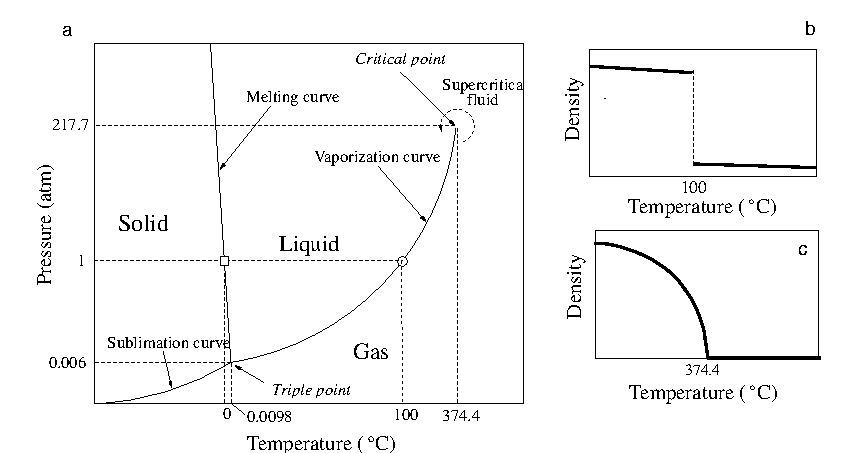
\includegraphics[scale=1.0]{chapters/ch2-crit/figs/water}
\end{center}
\caption{Phase diagram of water (a). Here, the three usual phases are
    distinguished, each separated from the other by a critical line. The phase
    transition that happens when the system traverse a line is characterized by
    a discontinuous jump in the density, as shown in (b) for the liquid-gas
    transition at $P=1$ atm. For $P=217.7$ atm however the same transition is
    continuous, as shown in (c). In the vicinity of this phase transition, at
    $T\approx374.4^\circ$C, the two phases become indistinguishable, and
    display a number of peculiarities. Systems in such state are called
    critical systems. Reproduced from~\cite{Sole2011}.}
\label{fig:water}
\end{figure}


\begin{figure}[h]
\begin{center}
    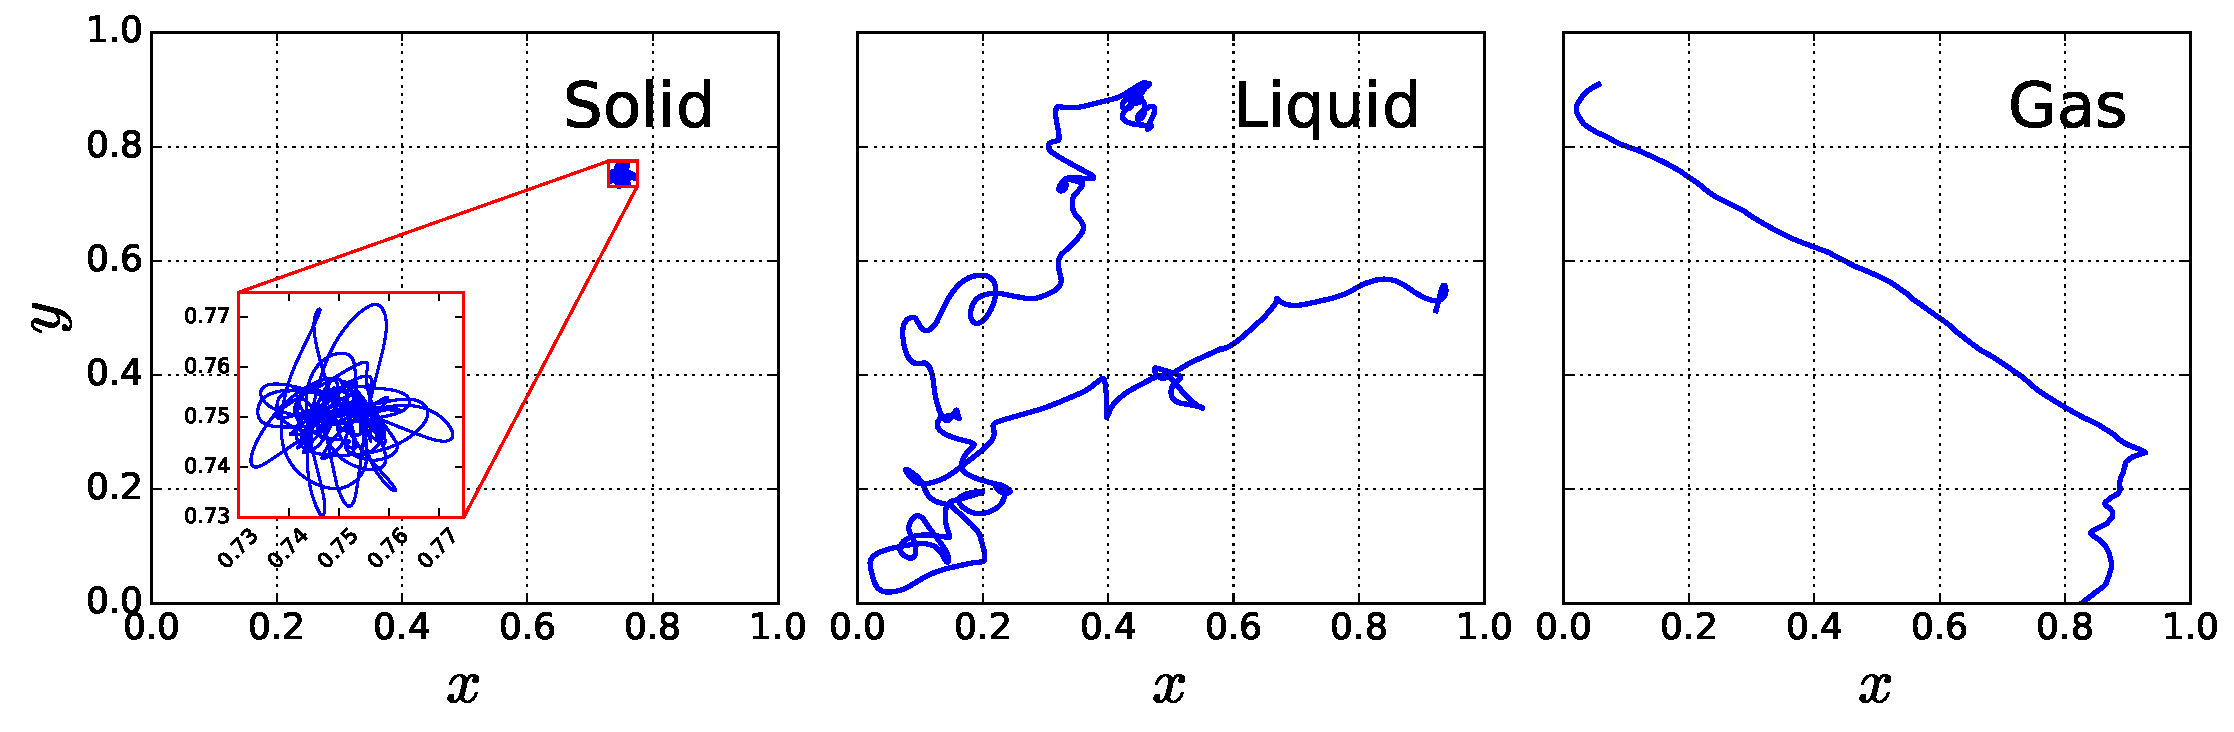
\includegraphics[scale=0.4]{chapters/ch2-crit/figs/phases}
\end{center}
\caption{How a system of particles behave in the three phases of matter. Here a
    simulation of 100 particles was done, but the trajectory of only one is
    shown. In the solid state the particles are confined to small region by
    the interactions of its neighbors. In the liquid state the particle is
    unconfined, but still interacts strongly with the other particles. In the
    gas state the kinetic energy of the particles is large enough that they
    barely interact with one another, making a ballistic trajectory until
    they make a head-on collision with another particle.}
\label{fig:phases}
\end{figure}


\begin{figure}[h]
\begin{center}
    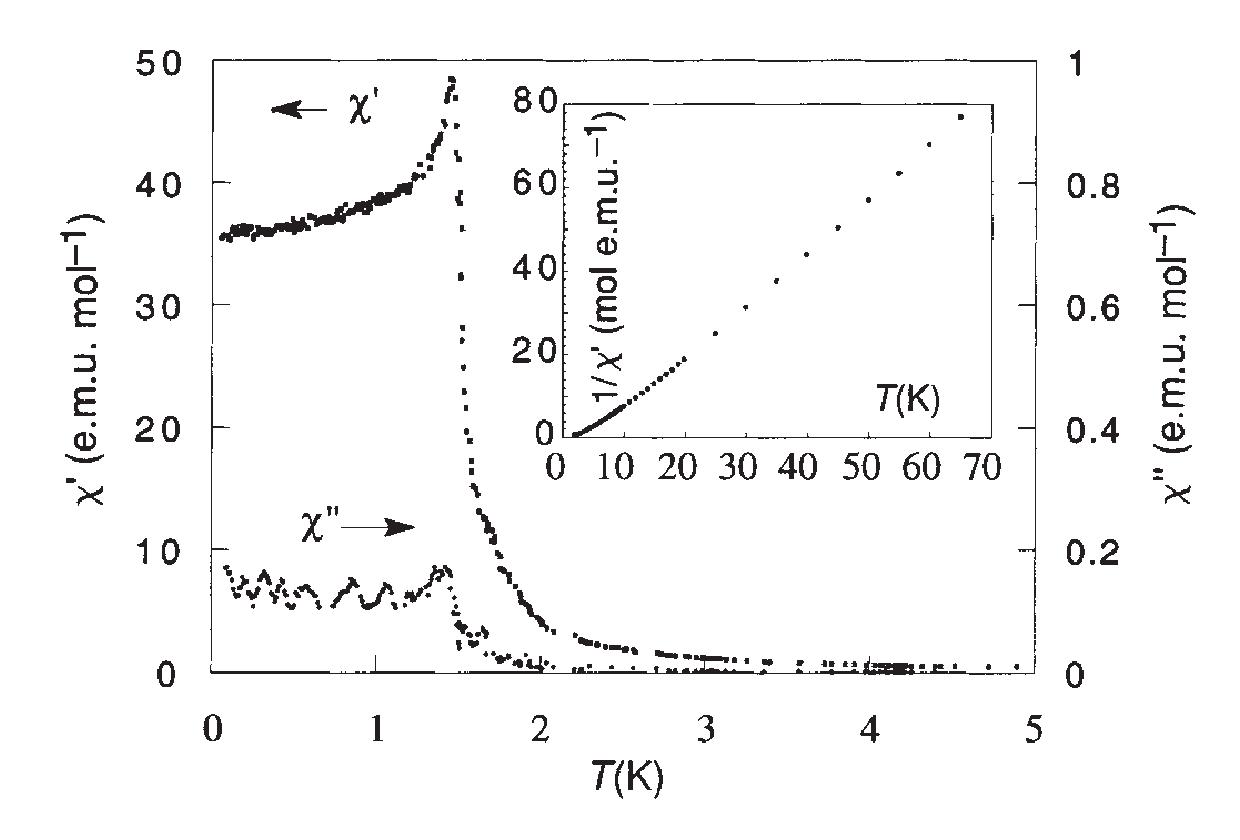
\includegraphics[scale=0.6]{chapters/ch2-crit/figs/suscep}
\end{center}
\caption{Example of a ferromagnetic transition in dupeyredioxyl. The graph
    shows a distinctive divergence in the magnetic susceptibility in the
    vicinity of the critical point $T_c\approx1.48$K. Reproduced
    from~\cite{Chiarelli1993}.}
\label{fig:suscep}
\end{figure}

\section{Classification of Phase Transitions}
\label{sec:classification}

In the literature, phase transitions usually fall in two categories: first
order and second order. But before we define each type it is good to do a
little thermodynamics refresher.

When we have a system defined by it's temperature $T$, pressure $P$ and
volume $V$, the thermodynamic properties of this system are determined
by a potential called \textit{free energy}.


\section{Ising Model}
\label{sec:ising}

For most of the first half of the 20th century, it was unclear whether the
formalism developed in statistical physics was enough to completely describe
phase transitions. That's because equations [\ldots] seems to behave neatly as
function of temperature. It wasn't until the work of Onsager in
1944~\cite{Onsager1944} that it became clear that the singularities appear only
in the limit of infinite particles, the thermodynamic limit.

It's impossible to understate the impact of the Ising model in the study of
phase transitions. It represents a golden standard because it unites an
elegantly simple setup with the fact it can be exactly solved in both one and
two dimensions, a claim very few models can make. Two of the most important
models, $O(n)$ and Pott's model, were constructed as generalizations of the
Ising model.

The system is composed of a number of classical spins $\{s_i\}$ that can take
one of two values $1$ or $-1$. The are arranged in a lattice and are allowed to
interact with its first nearest neighbors. The Hamiltonian of the systems is
given by
\begin{equation}
    \label{eq:ising}
    H\left(\left\{s_{i}\right\}\right) = 
        -J\sum_{\left\langle i,j\right\rangle}s_{i}s_{j}
        -h\sum_{i}s_{i}.
\end{equation}
Where $\sum_{\left\langle i,j\right\rangle}$ means a summation over all pairs
of nearest neighbors. If we assume $J>0$, then the first term of the
Hamiltonian favors the alignment of the spins, while the second one 
favors the alignment with an external magnetic field.

Just like the water example, the phase diagram of the Ising model is dependent
on two variables: the external magnetic field $h$ and the temperature $T$.

\begin{figure}
\begin{center}
    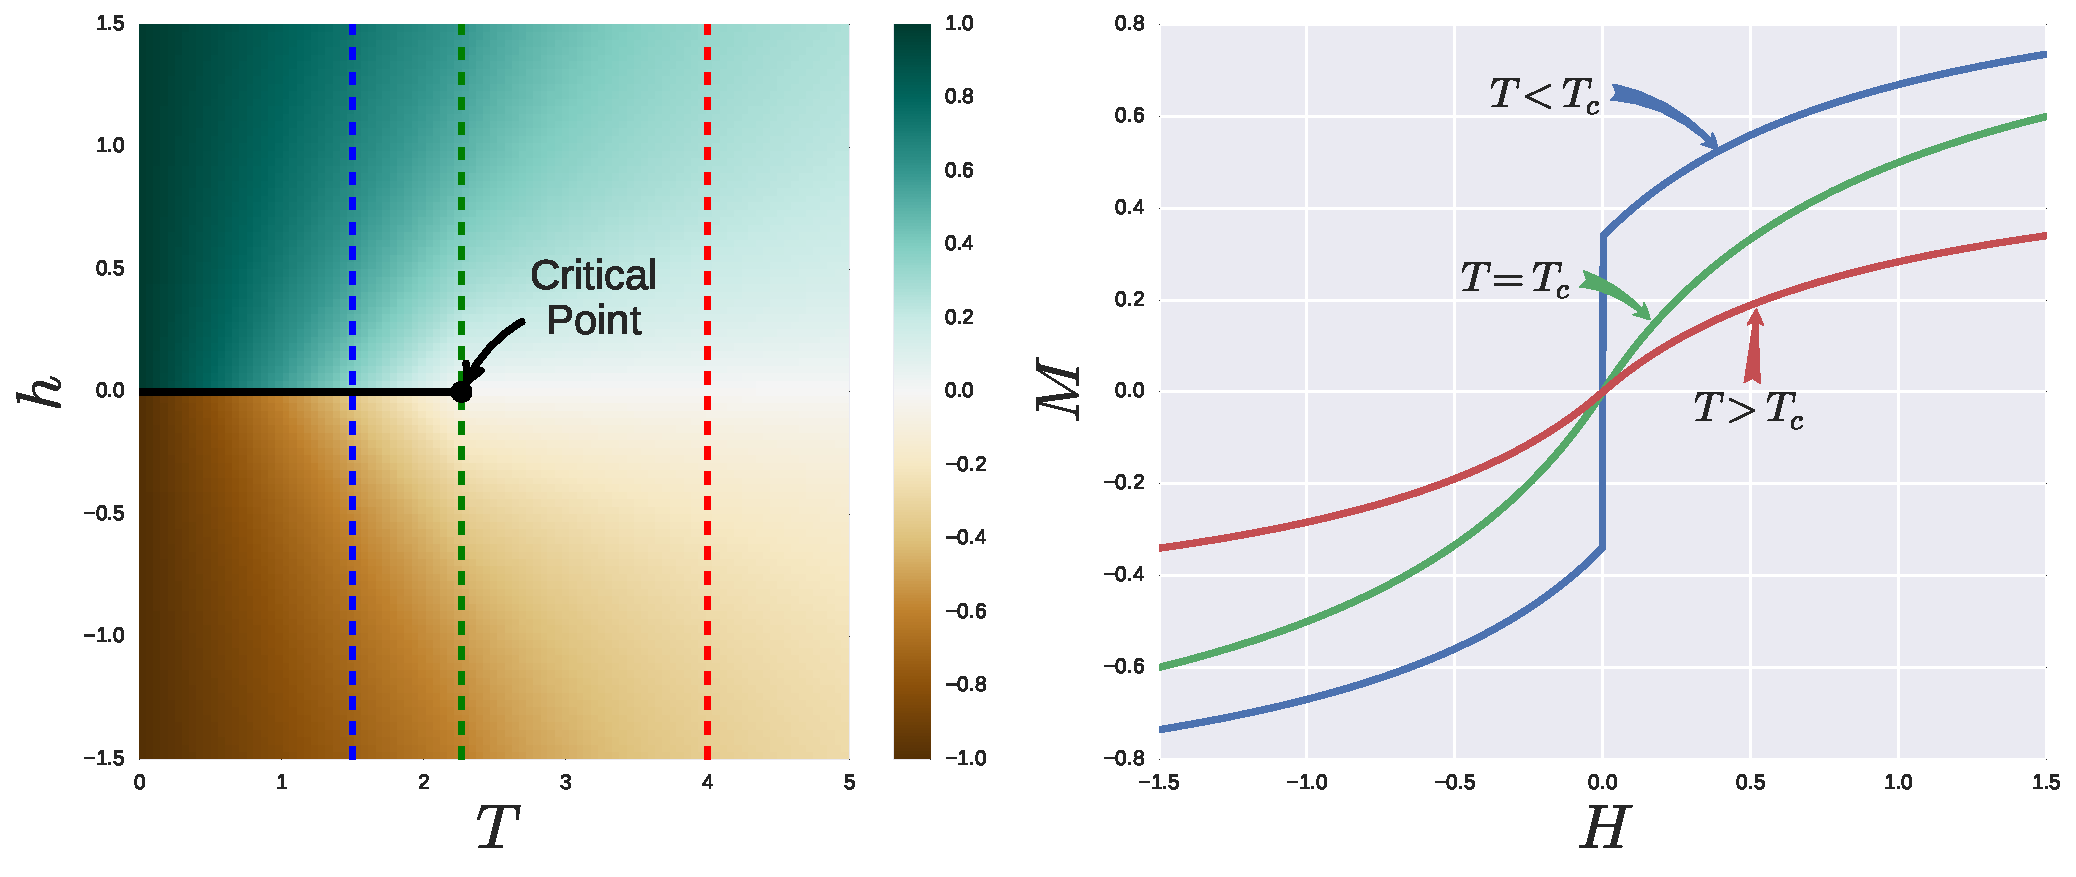
\includegraphics[scale=0.4]{chapters/ch2-crit/figs/ising_phase2}
\end{center}
\caption{The phase space of the Ising model (left). The color represents the
    spontaneous magnetization $M$ as a function of the external magnetic field
    $h$ and temperature $T$. The black line represents the critical line where
    the phase transition is of first order, which means the magnetization
    changes discontinuously like it's shown in the blue line. In the critical
    point the change is continuous and a second order phase transition takes
    place. Above the critical point no phase transition takes place.}
\label{fig:ising_phase2}
\end{figure}


\begin{figure}
\begin{center}
    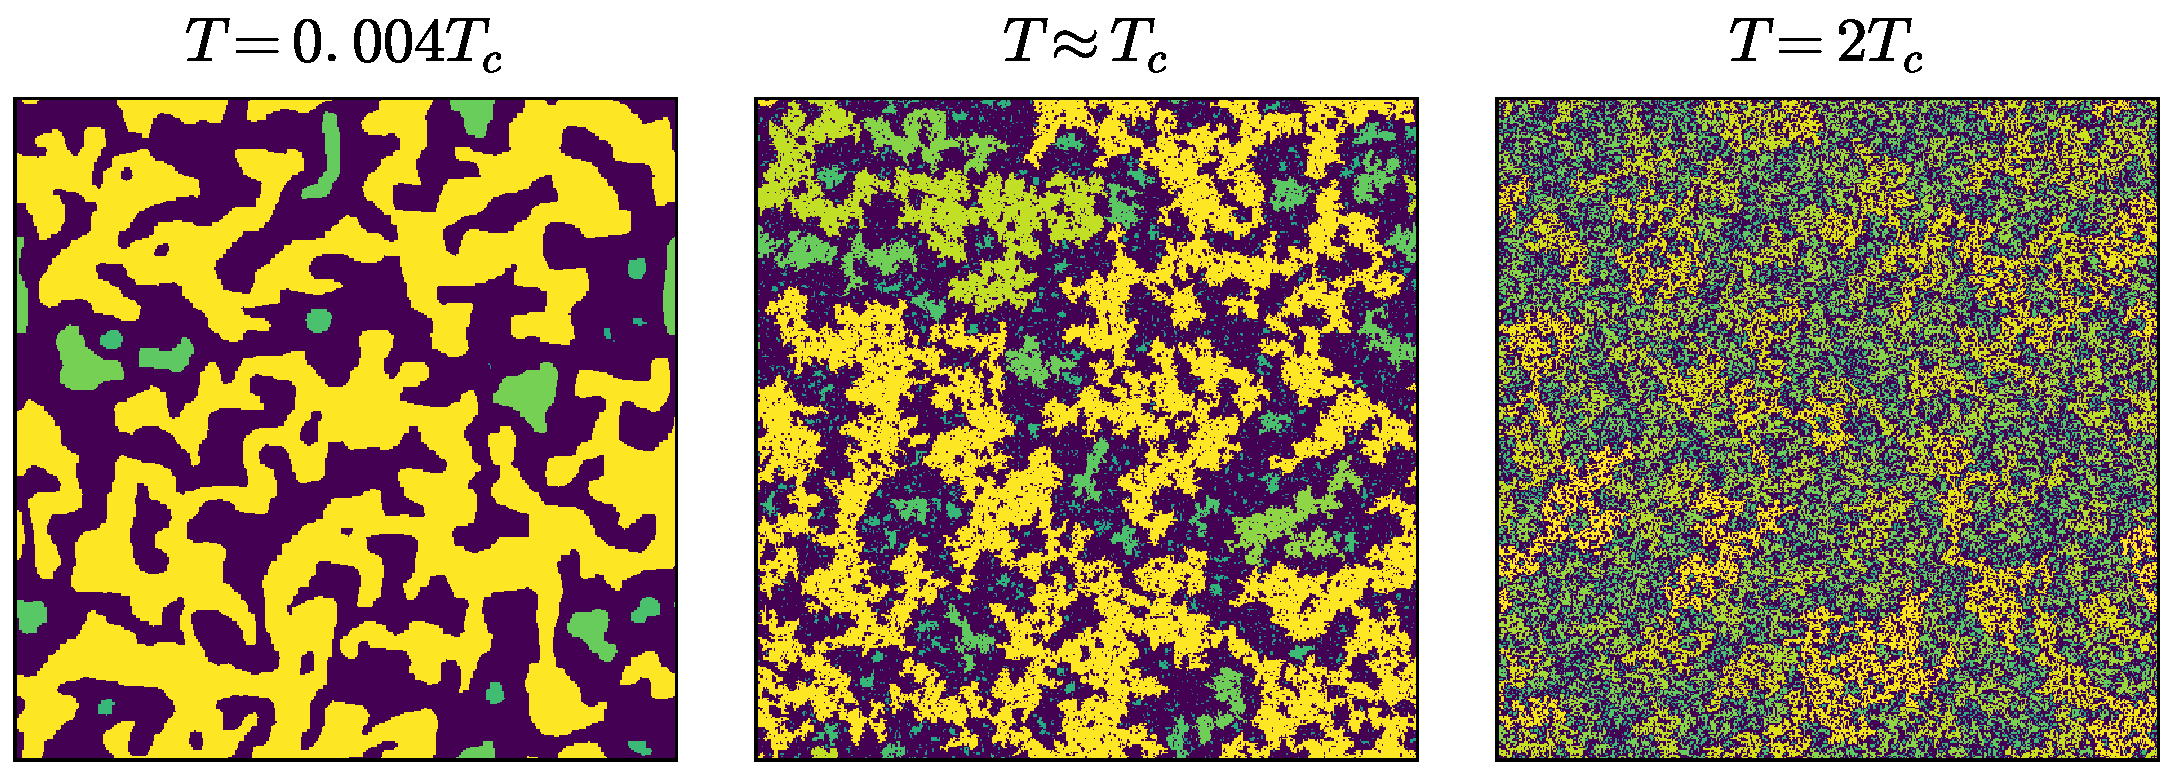
\includegraphics[scale=0.4]{chapters/ch2-crit/figs/ising}
\end{center}
\caption{Realizations of the Ising model with three different
    temperatures. The clusters of adjacent spin-up sites are colored according
    to how many sites belong to it. The subcritical regime is dominated by the
    large clusters. On the other hand, above the critical point, the system is
    dominated by thermal fluctuations, undermining cluster formation. At the
    critical point however, the clusters lack a characteristic length scale.
    One can observe that the image has a certain ``depth'' to it. This happens
    because clusters of all sizes are present, a mark of scale invariance,
    the most important property of critical systems.}
\label{fig:ising}
\end{figure}

\begin{figure}
\begin{center}
    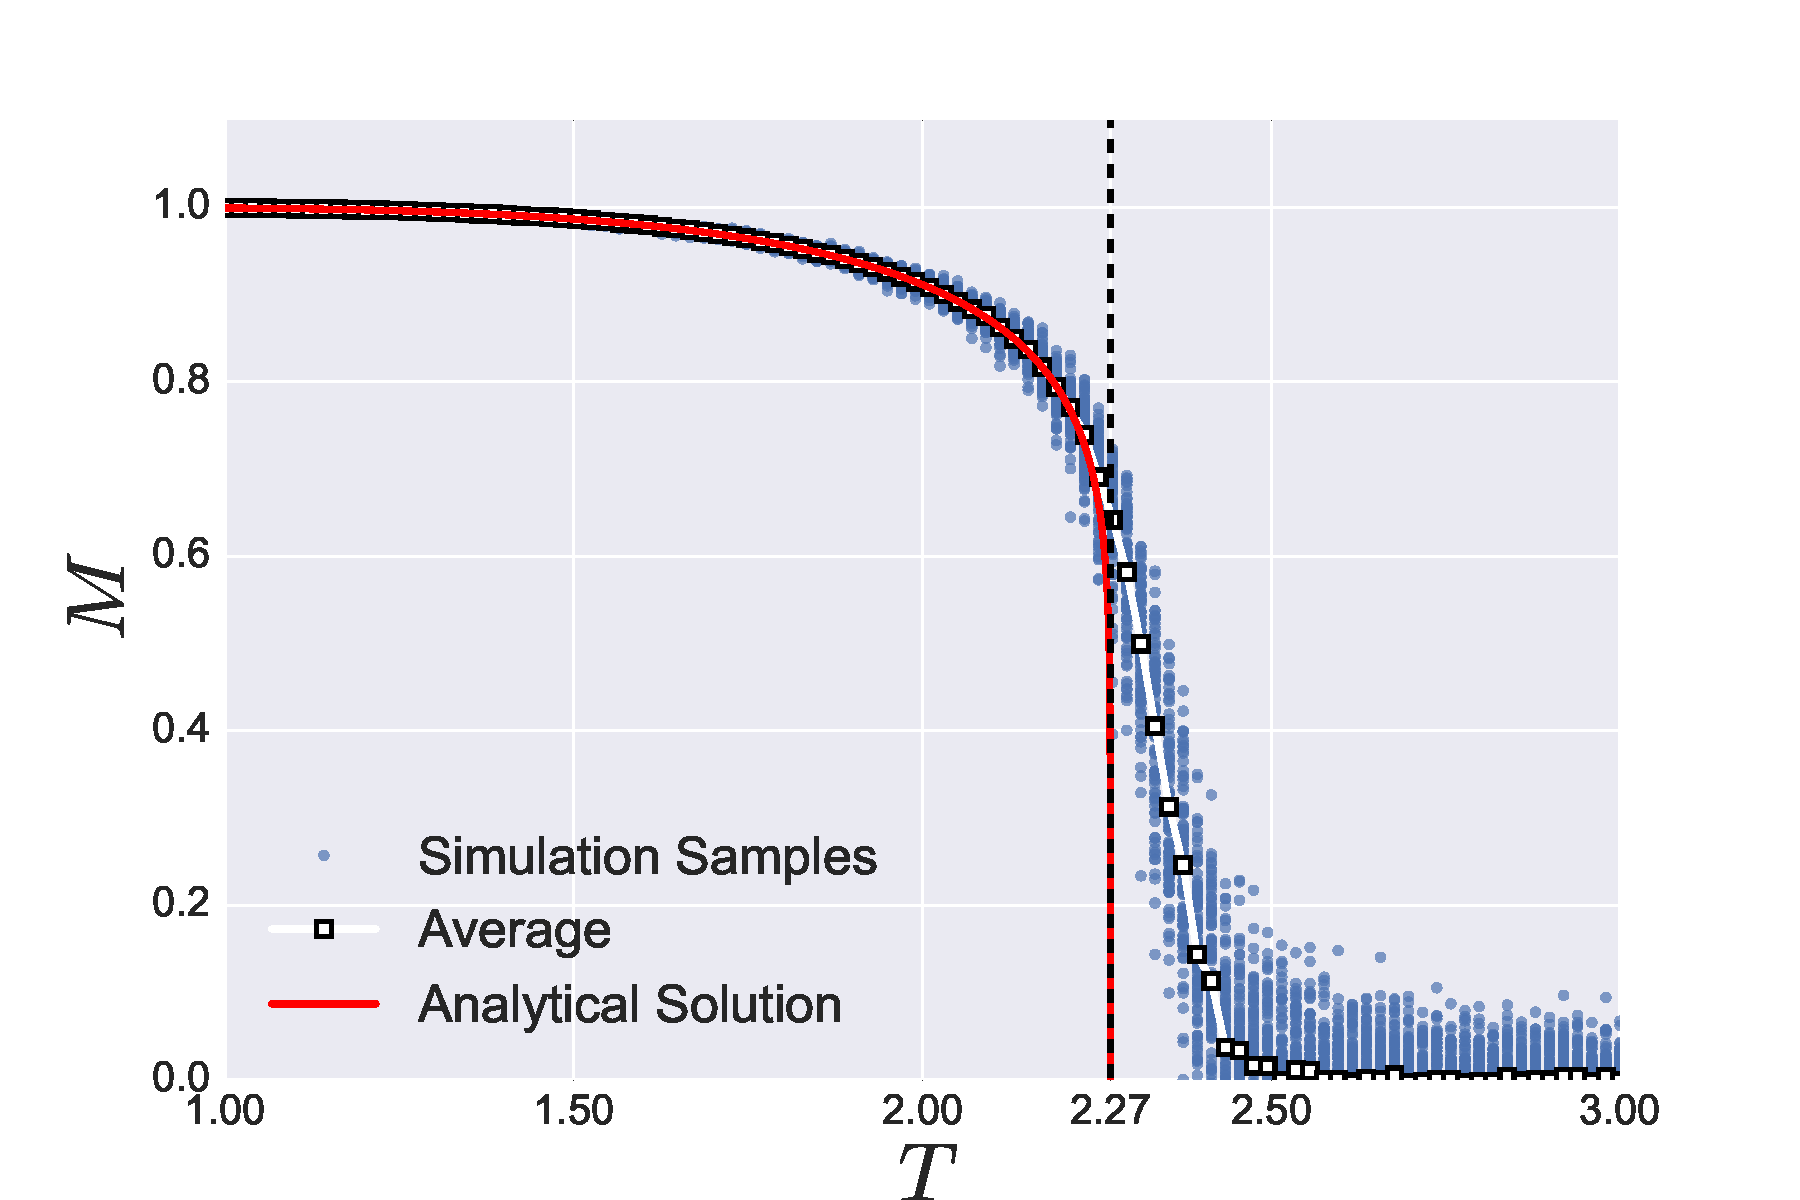
\includegraphics[scale=0.4]{chapters/ch2-crit/figs/ising_phase}
\end{center}
\caption{Spontaneous magnetization as a function of temperature for the Ising
    model. The simulations were performed in a $128\times128$ square lattice.
    As temperature rises, thermal fluctuations dominate the spin dynamics
    destroying the correlations. Above the critical temperature of
    $T_c=2/\log(1+\sqrt{2})\approx 2.269$ the value of $M$ should reaches zero,
    although due to finite size effects we still observe some magnetization
    beyond this point. The red line shows the illustrious solution
    developed by Onsager, where $M={[1-{(\sinh{2/T})}^{-4}]}^{1/8}$.}
\label{fig:ising_phase}
\end{figure}

Simulating the Ising model is particularly simple using the Metropolis-Hastings
algorithm. At each time step chose a random spin of the lattice and compute the
change in energy $\Delta E$ that would occur if you were to flip the spin. You
actually perform the flip if $\Delta E < 0$. If not, you should still accept
the flip randomly with probability $\exp(-\Delta E / T)$.

\section{Percolation}
\label{sec:perc}

While the Ising model certainly wins in terms of popularity, very few models
match the simplicity of percolation. Introduced in 1957 by Broadbent and
Hammersley, the passing decades saw its rise in prominence due to it's high
applicability ranging from transport in porous media to the propagation of
infectious diseases, with pretty much everything in between.

The original question Broadbent and Hammersley posed when coming up with
percolation was as fallows: if we submerge a large porous rock in water, will
the water penetrate the rock all the way to its center? In order to answer this
question they proposed the following model. We take a square lattice in any
number of dimensions wanted; this will be our rock.

\begin{figure}
\begin{center}
    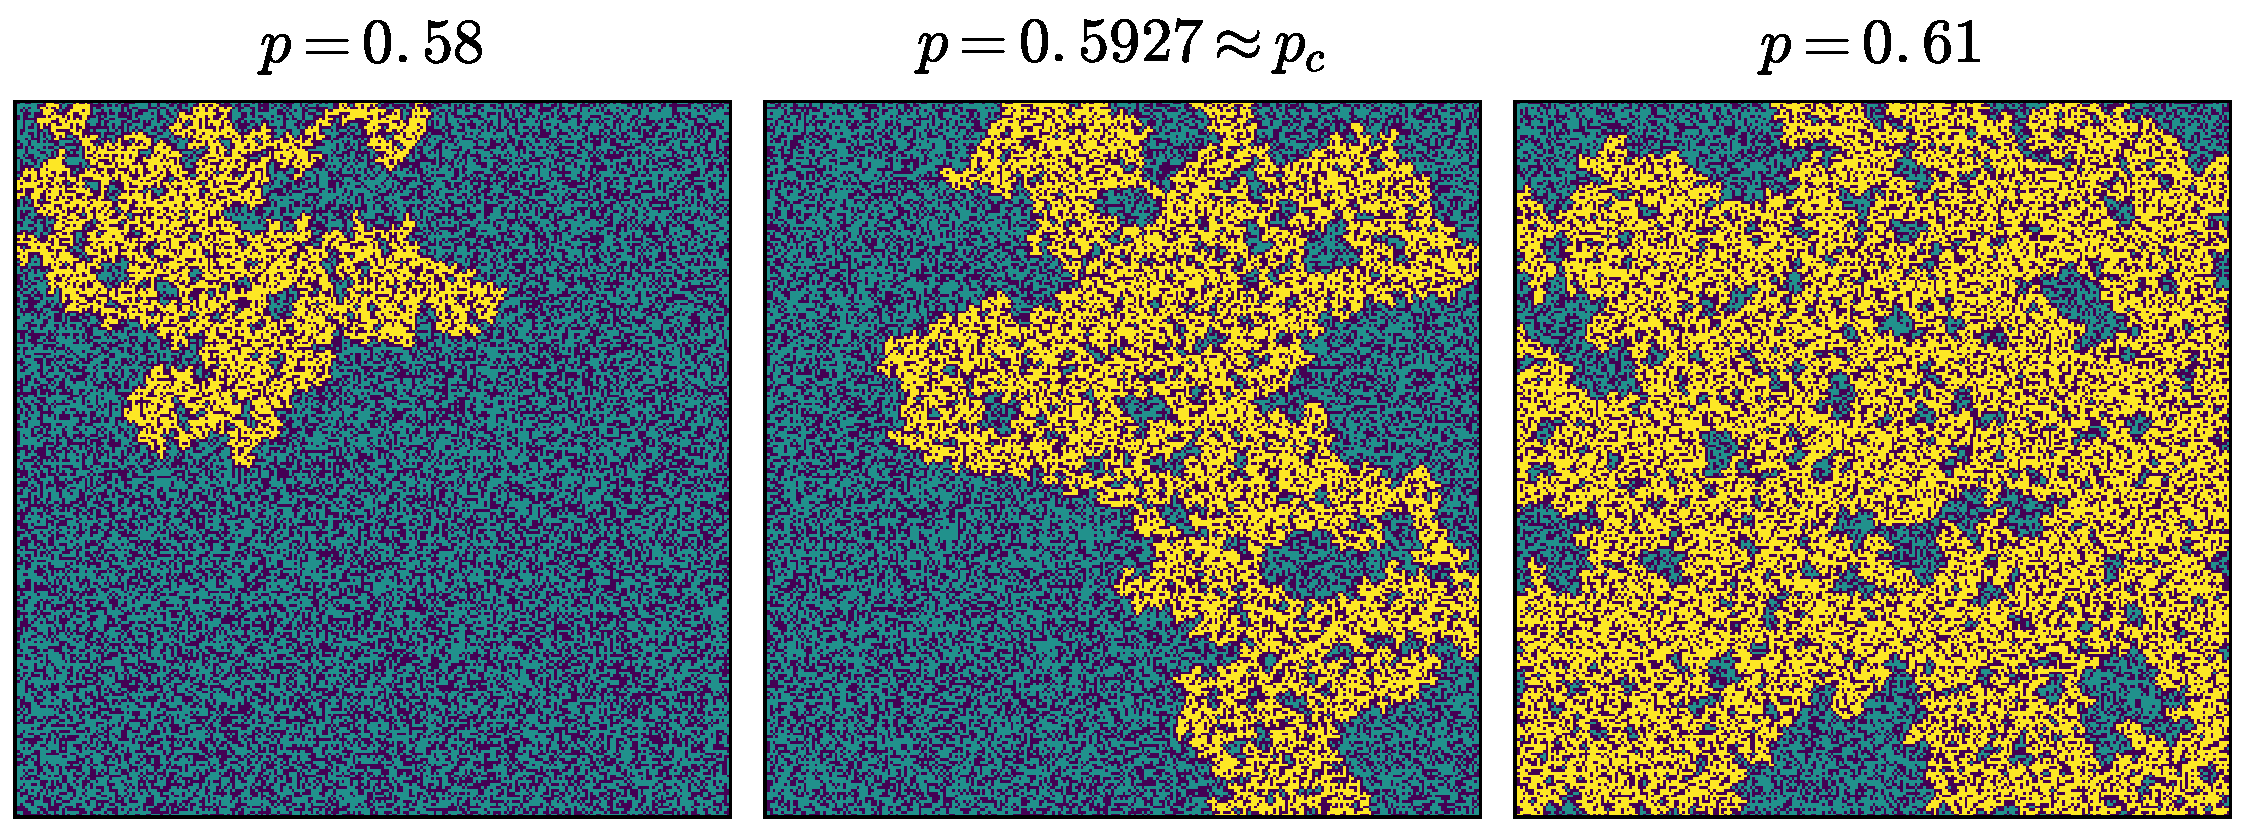
\includegraphics[scale=0.4]{chapters/ch2-crit/figs/isoperco}
\end{center}
\caption{Realizations of the percolation model in a square lattice with three
    different occupation probabilities $p$. Black sites are unoccupied, blue
    ones are occupied, and the largest cluster is painted yellow. For small
    values of $p$, there is no cluster that connects opposite sides of the
    systems. Above the critical point however, the largest cluster promotes a
    global connectivity, or, in terms of transport, the system becomes
    permeable.}
\label{fig:isoperco}
\end{figure}

\begin{figure}
\begin{center}
    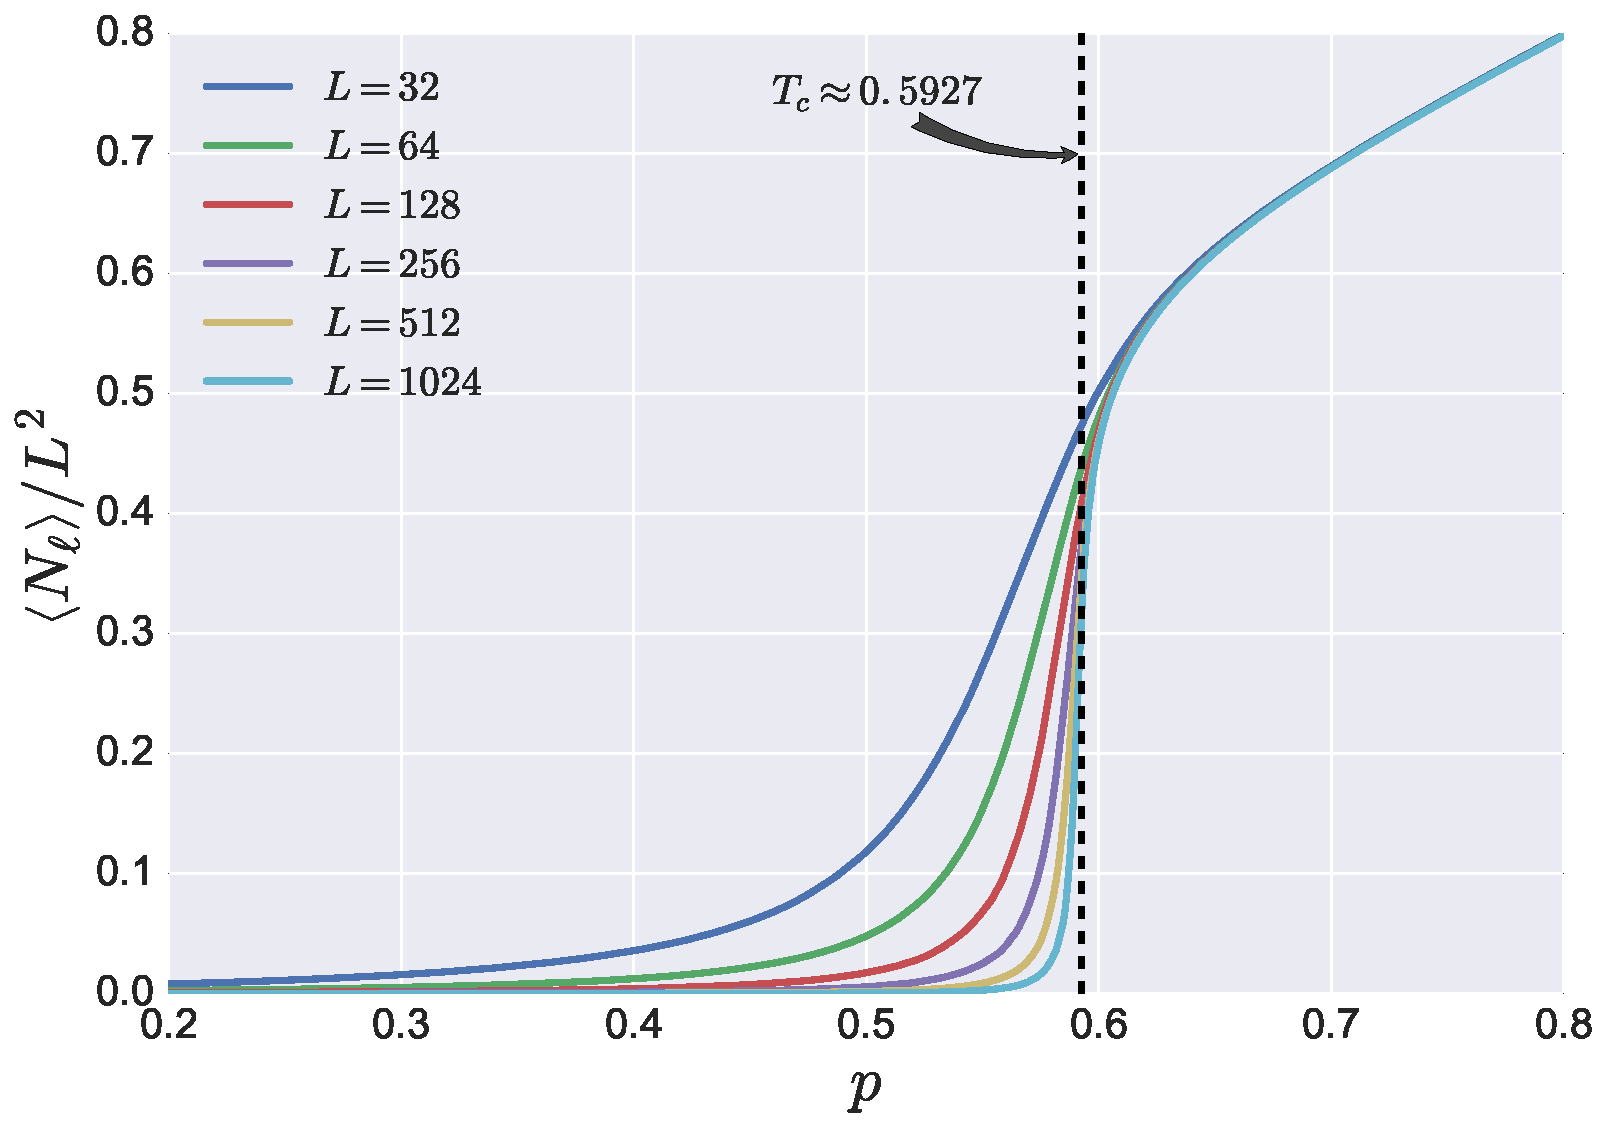
\includegraphics[scale=0.4]{chapters/ch2-crit/figs/isoperco2}
\end{center}
\caption{The order parameter of the percolation model as a function of the
    occupation probability for various system sizes. The order parameter here
    is defined as the fraction of the system occupied by the largest cluster.
    In the thermodynamical limit, the largest cluster have a finite size for
    $T<T_c\approx 0.592746$, that is, it occupies a negligible fraction of the
    system. Above the critical point the largest cluster is infinite and occupies
    a finite fraction.}
\label{fig:isoperco2}
\end{figure}

%\begin{figure}
%\begin{center}
    %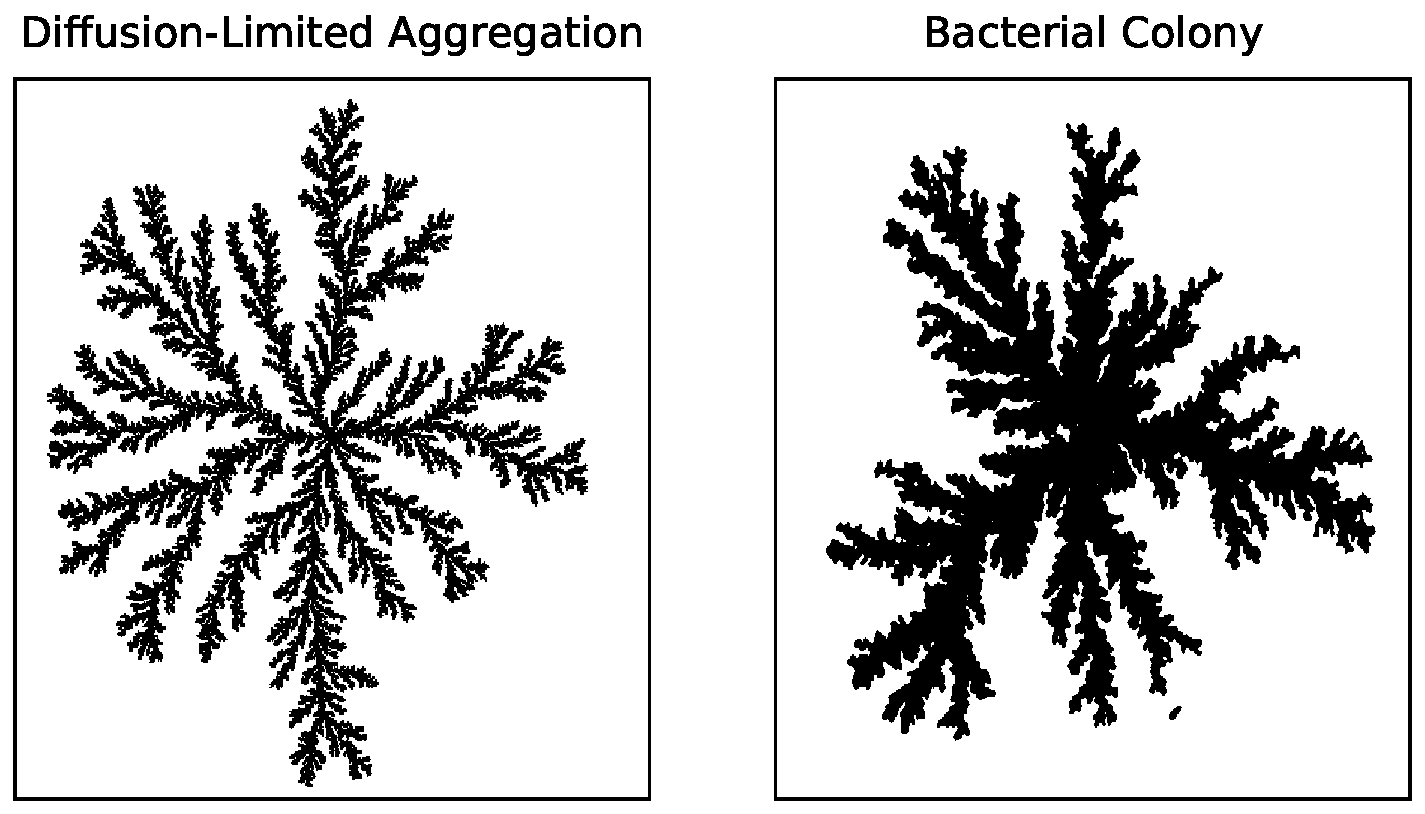
\includegraphics[scale=0.6]{chapters/ch2-crit/figs/bacteria}
%\end{center}
%\caption{Images taken from [???] and [???].}
%\label{fig:bacteria}
%\end{figure}


\section{Critical Exponents and Scaling Invariance}
\label{sec:scaling}

Let's illustrate using spin systems, composed by a collection of spins $\{s\}$
arranged in a lattice and interacting with one another and with an
external magnetic field $h$ according to a Hamiltonian
\begin{equation}
    \mathcal{H} \left(\{s\}\right)=
    \mathcal{H}_{int}\left(\{s\}\right) - h\sum_i s_i.
\end{equation}

The partition function is defined as 
\begin{equation}
    \mathcal{Z}=
    \sum_{\left\{ s_{i}\right\} }\exp\left(-\frac{\mathcal{H}}{T}\right)
\end{equation}
which is related to the free energy
\begin{equation}
    F=-T\log\mathcal{Z},
\end{equation}
from which we obtain the traditional relations used statistical mechanics
\begin{equation}
    C=-\frac{T}{\mathcal{N}}\frac{\partial^{2}F}{\partial T^{2}},
    \,\,\,\,\,\,
    M=-\frac{1}{\mathcal{N}}\frac{\partial F}{\partial h},
    \,\,\,\,\,\,
    \chi=\frac{\partial M}{\partial h}
\end{equation}

\begin{equation}
    G\left(r\right)=
    G\left(\left|\mathbf{r}_{j}-\mathbf{r}_{i}\right|\right)=
    \left\langle s_{i}s_{j}\right\rangle -
    \left\langle s_{i}\right\rangle \left\langle s_{j}\right\rangle 
\end{equation}
Here we suppose the system have translation invariance, so that the correlation
function depends only on the distance $r$ between two sites, and not on the
specific sites being analyzed.

\begin{equation}
    G\left(r\right)\sim r^{-\tau}e^{-r/\xi}
\end{equation}
where $\xi$ is called the \textit{correlation length}.

\begin{equation}
    \xi\sim\left|t\right|^{-\nu}\mbox{, where }h=0
\end{equation}

\begin{equation}
    \begin{array}{cccccc}
        C & \sim & \left|t\right|^{-\alpha} & \mbox{where } & h=0\\
        M & \sim & {\left(-t\right)}^{\beta} & \mbox{where } & t<0, & h=0\\
        \chi & \sim & \left|t\right|^{-\gamma} & \mbox{where } & h=0\\
        M & \sim & h^{1/\delta} & \mbox{where } & t=0
    \end{array}
\end{equation}

\section{Universality}
\label{sec:universality}

One of the most remarkable properties of complex system was first put forth by
Kadanoff in 1970~\cite{Kadanoff1971}.

Two systems that share the same set of critical exponents are said to belong to
the same universality class.
